\documentclass[preprint,  3p]{elsarticle}

\usepackage{csvsimple}
\usepackage{amssymb, amsthm}
\usepackage{amsmath}
\usepackage{subcaption}
\usepackage[T1]{fontenc}
\usepackage{babel}
\usepackage{wrapfig}
\usepackage{geometry}
\usepackage{fancyref}
\usepackage{lineno}
\usepackage{color}
\usepackage{nomencl}
\usepackage{tabularx}
\makenomenclature
\renewcommand{\nomlabel}[1]{\hfil #1\hfil}

\journal{}

\begin{document}
	\begin{frontmatter}
		\title{Computer Simulations of The Dynamics of Asymmetric Dimers in Optical Traps of Varying Polarization}
		
		\author[aff1]{Praveen Parthasarathi\corref{cor1}}
		\ead{praveen.parthasarathi@strath.ac.uk}
		
		\author[aff1]{Daniel Maciver}
		
		\author[aff1]{Leo Lue}
		
		\author[aff1]{Jan Sefcik}
		
		\author[aff1]{Mark Haw}
		
		\cortext[cor1]{Corresponding author}
		\affiliation[aff1]{organization={Department of Chemical Engineering,
				University of Strathclyde},
			addressline={75 Montrose Street}, 
			city={Glasgow},
			postcode={G1 1XL}, 
			country={Scotland}}
		
		\begin{abstract}
			% \justifying
			%
			We report on computer simulations of the dynamics of trapping, equilibrium positions and orientations of asymmetric microsphere dimers of varying size ratios in a single Gaussian beam Optical Trap of varying laser-polarization. We show that in case of a dimer, the trapping force profile deviates very quickly from a simple linear sum of forces on individual spheres as the size of the second sphere is increased and shows multiple axial-equilibrium positions for the case of larger bead closer to the laser focus as against the case of a smaller bead closer to the focus. Furthermore, we also investigate sustained rotations of dimers about their long-axis when trapped in a circularly polarized laser and study the effect of size-asymmetry on rotations. We hope these studies might be useful to researchers investigating colloidal aggregation and nucleation in optical traps and we also make a case for optically trapped dimers as rotors for use in experiments such as colloidal mixing.  
		\end{abstract}
		
		%\begin{graphicalabstract}
		%\begin{figure} [h]
		%	\centering
		%	\begin{subfigure}{0.45\textwidth}
			%		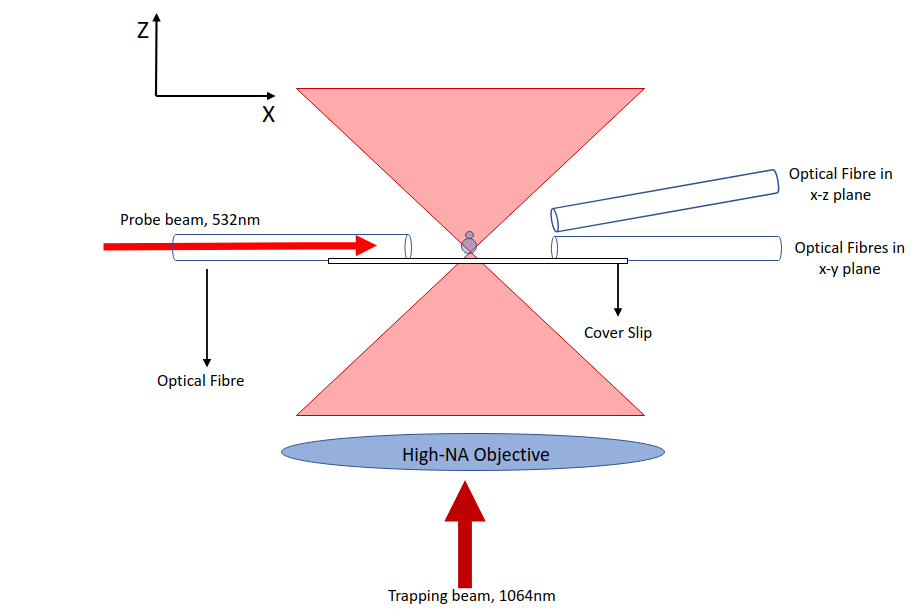
\includegraphics[width=\textwidth, height=0.25\textheight]{./Images/fig1a.png}
			%	\end{subfigure}
		%	\begin{subfigure}{0.45\textwidth}
			%		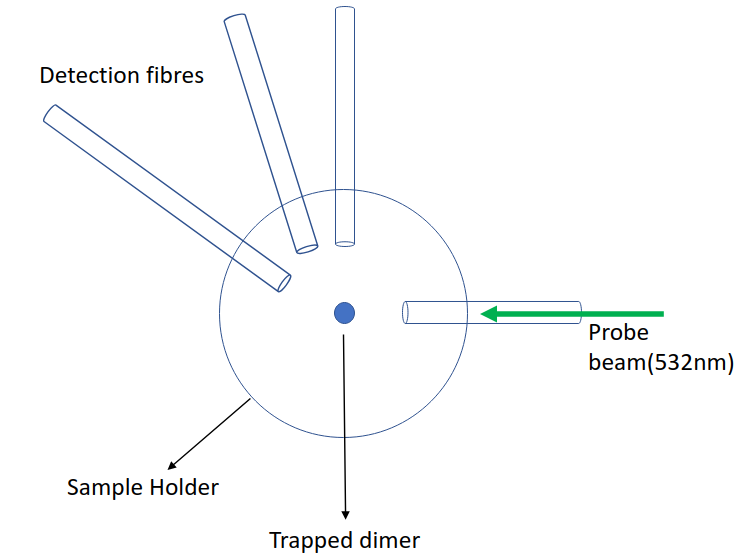
\includegraphics[width=\textwidth, height=0.25\textheight]{./Images/fig1b.png}
			%	\end{subfigure}
		%\end{figure}
		%\end{graphicalabstract}
		
		%\begin{highlights}
		%\item Asymmetric microsphere dimers can undergo complex dynamics including full inversions in the presence of a trapping potential, depending sensitively on the size ratio of the spheres making up the dimer.  
		%\item Orientations can be inferred from scattering signals through classification by a combination of neural networks and Bayesian inference. 
		%\item Signal error has a significant effect on the performance of the neural network, which can be countered via biasing of the prior distribution. 
		%\item Future applications include continuous processes where trapped particle characteristics such as size and shape are changing with time.  
		%\end{highlights}
		
		\begin{keyword}
			Optical Trapping \sep Brownian Dynamics \sep Micro-Rotors  \sep Colloids 
		\end{keyword}
		
	\end{frontmatter}

\section{Introduction}
Ever since their invention in 1986 by Arthur Ashkin \cite{Ashkin_1986}, Optical Traps or Optical Tweezers (OT) have been used extensively in colloidal physics \cite{Leonardo_2008, Koehler_2011, Curran_1999}. Of particular interest has been the use of a single trapped microsphere as a tracer to probe the rheological properties of the fluid of suspension \cite{Atakhorrami_2006}. However, while working with dense colloidal suspensions, one often ends up trapping more than one microbead in a Gaussian beam OT. Li and Arlt \cite{Li_2008} studied the case of two microspheres trapped in a single OT and opined that multiple trapped beads could be mistaken for a single trapped bead with altered trap stiffness. Theoretical studies on the case of two trapped microspheres by Xu et.al., \cite{Xu_2005} employed a ray-optics based model to show that the two trapped beads are brought into physical contact with each other by optical forces and they also calculated the axial equilibrium positions of the two trapped beads as a function of their size. Sheng-Hua et al \cite{ShengHua_2005} assumed that the two trapped beads experience different trap stiffnesses and went on to show that the trapped beads collide. Experiments in \cite{Praveen_2016} confirmed that the two trapped beads indeed experience different trap stiffnesses when trapped in a single Gaussian beam OT.

Besides multiple trapped beads, trapping and dynamics of asymmetric shapes have generated a lot of interest. Mihiretie et.al., \cite{Loudet_2014} studied the trapping of ellipsoidal microparticles and found that particles of aspect ratio ‘k’ greater than 3 and less than 0.3 exhibited oscillatory dynamics with a coupling between translation and rotation in the trap and those with aspect ratio outside this range exhibited less pronounced oscillations with the major axis pre-dominantly pointed along the laser propagation direction. Cao et.al., \cite{Curran_1999} performed T-Matrix based simulations of the trapping dynamics of nanowires and microcylinders in the Rayleigh regime and found that polarization dictated the final equilibrium orientation with the nanowires equilibrating with a large tilt angle about the laser propagation direction when the beam was linearly polarized and along the beam propagation direction in circularly polarized traps. Chetana D et, al., \cite{Chetana_2022} increased the complexity of the problem by considering an object with both shape as well as optical anisotropy in the form of a chicken Red Blood Cell (cRBC) and showed that the trapping dynamics and the final equilibrium orientation of the cRBC was decided by the beam polarization with the cell showing a dual reorientation behaviour in a linearly polarized trap and a partial second reorientation in a circularly polarized trap.  
In this work, we extend the Brownian dynamical simulations carried out by Vigilante et.al., \cite{Vigilante_2020} to the case of asymmetric dimers. We begin by showing that the optical force on a microsphere-dimer quickly deviates from a simple sum of forces on two spheres and thus underscore the relevance of the choice of mstm, a well-established package for calculating light scattering from a cluster of spheres \cite{Mackowski_2011} and within it ott, a well-established toolbox for computing forces and torques in an OT \cite{Nieminen_2007}.  We show validations of the dynamical simulations for the case of a single trapped bead in both linear and circularly polarized traps with the suspension medium being water at room temperature. We then reproduce the results for dynamics of a symmetric dimer in \cite{Vigilante_2020} as further validation of our codes. We organize our results into 3 sections with the focus on axial and orientation trapping equilibria for different size-ratios of the dimers in the first section, determinations of equilibrium orientations and equilibrium positions of various dimers with varied initial conditions of orientation and position in linearly and circularly polarised traps, Finally, we report interesting rotational dynamics of dimers seen only when the light is not linearly polarised. We hope that our results could inform studies on colloidal aggregation and help design rotors for use in applications such as lab-on-a-chip and micromachines.        

\newpage
\bibliography{dimer_bib} 
\bibliographystyle{ieeetr}

\section{Methodology}
\paragraph{Simulating motion within an optical trap}
We assume the dimers to be low-Reynold’s number objects and write down their dynamics within the trap using the Langevin equation:
\begin{align}
	\label{eq:langevin}
	\frac{dx(t)}{dt}=\frac{F(x)}{\gamma}+\sqrt{2D}\eta_x(t)
\end{align}

Where $F(x)$ is the optical force directed towards the focal point of the laser However, this is only accurate when close to the equilibrium position, if we wish to probe the phase space we need a means of computing the optical forces for any position or orientation. Fortunately, Vigilante et al \cite{Vigilante_2020} have already built the ground work for simulating multi-sphere trapping. This work is an extension of the simulation work conducted by \cite{Vigilante_2020} into multi-sphere objects; their paper already has an excellent breakdown of the mathematics that go into calculating the optical and hydrodynamic forces, as such we will only refer to the mathematical methodology when necessary or when our work diverges from \cite{Vigilante_2020}. For simulating asymmetric objects, in which translation and rotation dynamics are coupled, it is useful to have two separate reference systems: The laboratory frame, which refers to the larger system centred at the focal point of the trapping laser; and the particle reference frame which defines the positions of individual spheres, in the case of a dimer the spheres are positioned so that the centre of diffusion is at the origin of the particle reference frame. The axis of the particle reference frame is used to define the orientation of the dimer; with Uz intersecting the centres of the two spheres; any rotations are applied to the reference axis so that the orientation is preserved.

The code combines the optical force calculation code from Optical Tweezer Toolbox (ott) and the T-matrix calculations from Multi-Sphere T-Matrix (mstm); after initializing the target object mstm calculates its T-matrix before returning the T-matrix object to ott to calculate the optical forces and torques as well as the hydrodynamic forces due to the Brownian force. This circumvents the limitations of both ott and mstm; mainly that ott struggles to model the T-matrix of multi-shape objects that experience internal scattering, and that mstm cannot model scattering from lasers with a high NA commonly used in optical trapping. After calculating the total force and torque in the laboratory frame they are scaled down to the particle reference frame, where the reference axis is rotated appropriately before then displacing the object in the laboratory frame to update its position.  

\begin{figure}[h]
	\centering
	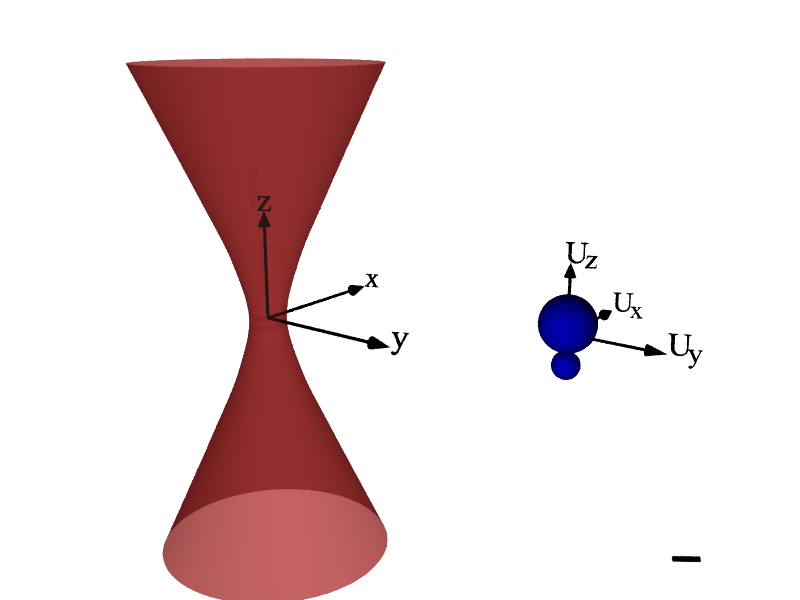
\includegraphics[width=0.75\textwidth]{./Images/Lab_frame.png}
	\caption{\label{fig:lab_frame}
		%
		Render of trapping beam and a dimer (size ratio 2) with respective laboratory frame and particle reference frame. The laboratory frame origin is set at the focal point of the Gaussian beam. The particle reference axes are used to set the relative positions of each sphere, the axes are centred on dimer's centre of diffusion and used to describe the dimer’s orientation. Scale bar in bottom right corner represents 1 $\mu$m
		%
	}
\end{figure}

The Brownian OT code from Vigilante has code for simulating both dimers, and sphere clusters; the former is only capable of processing symmetric dimers with no ability to freely tune the size of each sphere. To simulate the behaviour of asymmetric dimers we modelled the entity as a sphere cluster consisting of two spheres tangentially attached, the larger sphere is defined as sphere 1 with radius ‘$r_1$’ the second sphere is then defined by the size ratio $\lambda$ so that $r_2 = \lambda r_1$.  Knowing the size ratio is critical for defining the dimer’s centre of diffusion and also for appropriately scaling its diffusion tensor. The diffusion tensor is calculated from Nir and Acrivos \cite{Nir_1973} work into arbitrary shaped spherical objects; where they write the diffusion tensor as a 6x6 matrix, when the dimer is symmetric only the central diagonal is non-zero. However, for asymmetric dimers the forces on the spheres are unequal resulting in stress build up along the dimer’s long axis, the diffusion tensor is then given as:
\begin{align}
	\label{eq:diffusion}
	D=\frac{k_BT}{\pi\mu}\left[
	\begin{matrix}
		a_1 & 0 & 0 & 0 & d_1 & 0\\
		0 & a_1 & 0 &-d_1 & 0 & 0\\
		0 & 0 & a_1+a_2 & 0 & 0 & 0\\
		0 & -d_1 & 0 & b_1 & 0 & 0\\
		d_1 & 0 & 0 & 0 & b_1 & 0\\
		0 & 0 & 0 & 0 & 0 & b_1+b_2\\
	\end{matrix}\right]
\end{align}
Where the constants are spline fitted from the results of [14], due to the dimer’s asymmetry the friction coefficient – which is related to the diffusion coefficient – is different depending on the axis the fluid is flowing parallel to. The Brownian displacements and rotations are generated at random in proportion to the diffusion tensor. 
\paragraph{Finding equilibrium positions}
In order to determine the equilibrium trapping locations of an arbitrary multi-sphere cluster we need to be able to compute the optical force at any position and orientation. The optical forces can be computed by a summation of the incident and scattered beam expansion coefficients; the z-axis force is given below:

\section{Results and Discussion}
Trapping forces on a sphere are often written as the rate of change in momenta of incident and scattered beams \cite{Nieminen_2007}. We show in Fig. [1], the axial-force on a single trapped polystyrene micro bead of varying radii as the bead is moved along the z-axis computed using the Optical Tweezer Toolbox ott under a linearly polarised trap generated with an objective lens of NA 1.2 and wavelength 1064nm. For the case of a dimer, we use mstm to compute the scattered fields and ott to compute the forces and torques consequent of the scattering processes. It may seem reasonable to write down the force on a dimer as the sum of forces on two beads that make up the dimer with positions of the centre of each bead measured from the beam focus. We put this approximation to test in Fig [2] where we compare it with a rigorous calculation of the force using mstm and ott and see it fail as soon as the second bead starts being a 10th in radius of the first bead. This makes the case for use of packages like mstm which are dedicated to computing multi-sphere scattering. We adopt the python codes in \cite{Vigilante_2020} to simulate Brownian dynamics of a dimer made of spheres of diameter 0.8micron trapped in a left-circularly polarised light of power 5mW and the spheres are assumed to be made of polystyrene of refractive index 1.58 with water of index 1.33 at 295K as the medium of suspension. Optical forces and torques on this dimer are shown in Fig [3].  and rotation frequency of the dimers as a function of the ratio of the Stokes vector element $S_3/S_0$ is shown in Fig. [4]. We see very good agreement of these results with those reported in \cite{Vigilante_2020}. 

\subsection{Axial forces and Equilibrium positions}
We explore the trapping landscape by plotting out the trapping force as the dimer is moved along the z-axis and see that for the case of large-bead-over-small, there are multiple trapping equilibria compared to the case of small-bead-over-large as seen in Fig [4] and Fig [5]. In all these calculations, we maintain the radius of one of the beads making up the dimer at 1micron and vary the size of the other bead to 500nm, 250nm, and 100nm respectively in the case of size-ratios 2, 4, and 10. In Fig. [6] we plot out the force curve for a symmetric dimer with the size of each sphere equal to 1 $\mu m$.  


\end{document}